\documentclass[12pt, twoside]{article}
\usepackage{jmlda}
\usepackage{NotationStyle}

\usepackage{pdfpages}
\usepackage{wasysym}
\usepackage{amsmath, amsfonts, amssymb}

\usepackage{graphicx}
\usepackage{longtable}
\usepackage{booktabs}

\newcommand{\hdir}{.}

\newtheorem{hop}{Гипотеза}

\let\local\relax
\DeclareMathOperator {\local}{a}

\begin{document}

\title
    {Поиск границ радужки методом круговых проекций} % окончательное ли название?
\author
    {А.\,А.~Баженов, И.\,А.~Матвеев} % основной список авторов, выводимый в оглавление
\email
    {bazhenov.aa@phystech.edu; ivanmatveev@mail.ru}
%\thanks
%    {Работа выполнена при
%     %частичной
%     финансовой поддержке РФФИ, проекты \No\ \No 00-00-00000 и 00-00-00001.}
%\organization
%    {$^1$Организация, адрес; $^2$Организация, адрес}
\abstract
    {В работе рассматривается задача приблизительного нахождения границ радужки глаза. Входными данными являются изображение и считающееся известным положение зрачка глаза. Для нахождения границ зрачка и радужки используется нейронная сеть, для достижения максимальной производительности алгоритма используется предварительная обработка данных. Работа алгоритма проверена на базе изображений.
	
\bigskip
\noindent
\textbf{Ключевые слова}: \emph {}

}

%данные поля заполняются редакцией журнала
%\doi{10.21469/22233792}
%\receivedRus{01.01.2017}
%\receivedEng{January 01, 2017}

\maketitle
\linenumbers

\section{Введение}
Жизнь современного человека неразрывно связана с большим количеством аккаунтов, к каждому из которых необходим надежный способ аутентификации. Обзоры [1, 2] отмечают становление популярности биометрических способов идентификации человека относительно классических, таких как использование паролей. Обзор [2] особо выделяет методы, основанные на распознавании радужки, как позволяющие достигнуть высокой точности распознавания. Первичное выделение регионов на изображении глаза человека является одним из важнейших этапов персональной идентификации. В статье [3] описана общая схема работы системы сегментации изображения глаза: нахождение приблизительной позиции зрачка и последующее нахождение границ зрачка и радужки, с возможным итеративным уточнением.

В [3, 4] для реализации этапа первоначального определения границ радужки  используется метод круговых проекций. Круговая проекция яркости~--- интеграл градиента яркости изображения по окружности, имеющей центр в предполагаемом центре зрачка, либо по ее дуге. По предположению из [4], найдя точку локального максимума зависимости круговой проекции яркости от радиуса окружности, можно найти радиус границы радужки. Однако на яркость изображения в районе границы может оказываться влияние затемнения от ресниц и других элементов лица, что делает возможность эвристических алгоритмов, используемых в [3, 4] ограниченным.

Целью работы является исследование методов, которые возможно использовать для обработки результатов подсчета круговых проекций, причем более устойчивых к влиянию внешних факторов, чем эвристические алгоритмы. Один из таких методов~--- использование нейронной сети. Именно этом метод было решено исследовать в рамках работы.

\section{Постановка задачи}
\subsection{Модель системы нахождения границ радужки}

Рассматриваются данные в виде растрового изображения глаза $M$. Изображение представляет из себя зрачок~--- круг с центром в точке $\begin{pmatrix}P_x & P_y\end{pmatrix}\T$ и радиусом $P_\text{R}$, окруженный радужкой~--- кругом с центром в точке $\begin{pmatrix}I_x & I_y\end{pmatrix}\T$ и радиусом $I_\text{R}$, часть которого может отсутствовать на изображении. В дальнейшем будем называть $P_\text{R}$ \textit{радиусом границы зрачка}, а $I_\text{R}$~--- \textit{радиусом границы радужки}. Помимо зрачка и радужки, на изображении присутсвуют посторонние элементы.

Модель системы нахождения границ радужки представляется отображением
\[f\!: \quad M \mapsto \begin{pmatrix}\widehat{P}_x & \widehat{P}_y & \widehat{P}_\text{R} & \widehat{I}_x & \widehat{I}_y & \widehat{I}_\text{R}\end{pmatrix}\T.\]
В работе рассматривается задача приблизительного нахождения границ, поэтому малые отклонения не должны штрафоваться, а большие отклонения должны штрафоваться сильно. Рассмотрим кусочно-линейную функцию
\[
h_{\alpha, \beta}(t) = \begin{cases}0, &x < \alpha, \\ x - \alpha, &\alpha \leqslant x < \beta, \\ (\beta - \alpha) + 5\cdot (x - \beta), & x > \beta.\end{cases}
\]
Используемая в работе функция потерь~--- результат композиции функции $h_{\alpha, \beta}$ и функции относительного отклонения
\[
L_{\alpha, \beta} (x, y) = h_{\alpha, \beta}\left(\frac{|x-y|}{y}\right).
\]
По экспертным соображениям, были выбраны значения $\alpha = 0.1$ и $\beta = 0.2$. Рассматривается задача оптимизации
\begin{equation}\label{mainproblem}
\sum_{i=1}^n L_{\alpha, \beta} \left(\widehat{P}_\text{R}(i), P_\text{R}(i)\right) + L_{\alpha, \beta} \left(\widehat{I}_\text{R}(i), I_\text{R}(i)\right) \to \min_{f\in \mathcal{F}},
\end{equation}
вид множества допустимых моделей $\mathcal{F}$ описывается в разделе 2.3.

\subsection{Метод круговых проекций}
Обозначим $\vec{x} = (x, y)$~--- точку на изображении, $b(\vec{x})$~--- яркость изображения в этой точке, $\vec{g}(\vec{x}) = \nabla b(\vec{x})$~--- градиент яркости. Согласно предположению, указанному в статье [4], точки, лежащие на границе радужки либо зрачка, должны удовлетворять условию, описываемому индикаторной функцией:
\[
v_U(\vec{x}) = \begin{cases}1, & \parallel \vec{g} \parallel > T_1 \land \frac{(\vec{x}, \vec{g})}{\parallel x \parallel \cdot \parallel g \parallel} > T_2 \land \vec{x} \in U, \\ 0, & \text{ иначе,}\end{cases}
\]
где $T_1$ и $T_2$~--- некоторые пороговые значения, а $U$~--- квадрант, то есть одно из множеств точек плоскости:
\[
U = \begin{cases}L\!: & |x| > |y| \land x < 0, \\ R\!: & |x| > |y| \land x > 0, \\ B\!: & |x| \leqslant |y| \land y < 0, \\ T\!: & |x| \leqslant |y| \land y > 0.\end{cases}
\]

Для аккумуляции значений индикаторных величин вводится следующее понятие. Пусть зафиксирован некоторый квадрант $U$. Тогда \textit{круговой проекцией яркости по окружности радиуса $r$} называется следующая величина:
\[
\Pi_U(r) = \frac{1}{2\pi r} \sum_{r-0.5 \leqslant \parallel x \parallel \leqslant r + 0.5} v_U(r).
\]

\subsection{Ограничение на множество моделей}

Рассмотрим задачу нахождения радиусов границ радужки и зрачка при известном приблизительном положении центра зрачка. Обозначим $\Pi$~--- процедуру подсчета круговых проекций яркости. При решении задачи~\eqref{mainproblem} рассматриваются только модели, обрабатывающие значения круговых проекций нейросетевым способом,
\[
\mathcal{F} = \left\{f = \varphi \circ \Pi \mid \varphi(t) = \sigma_k\left(W_k\T \sigma_{k-1}\left(\ldots \sigma_1\left(W_1\T t\right)\ldots\right)\right)\right\}\!.
\]
При фиксированной архитектуре $\varphi$, то есть при фиксированных $k$ и функциях активации $\sigma_1, \ldots, \sigma_k$ решается задача оптимизации среднеквадратичного отклонения
\begin{equation}\label{secondproblem}
\frac{1}{n}\sum_{i=1}^n \left(\widehat{P}_\text{R}(i) - P_\text{R}(i)\right)^2 + \left(\widehat{I}_\text{R}(i) - I_\text{R}(i)\right)^2 \to \min_{W_1, \ldots, W_k}.
\end{equation}

\section{Нахождение радиусов границ}

Пусть считается известной зависимость значения круговой проекции яркости от радиуса $\Pi_U(r)$. Рассмотрим некоторые значения радиусов $r_1$ и $r_2$. Исходя из определения круговой проекции делается предположение:
\begin{hop}
Если выполнено неравенство $\Pi_U(r_1) > \Pi_U(r_2)$, то вероятность наличия круговой границы радиуса $r_1$ больше, чем вероятность наличия границы радиуса $r_2$.
\end{hop}

Практика показывает, что для произвольных значений $r_1$ и $r_2$ гипотеза 1 неверна. Однако гипотеза не опровергается экспериментальными данными в локальном случае, то есть при выборе некоторой малой величины $\varepsilon$ утверждение гипотезы 1 не опровергается при выполнении
\[
|r_1-r_2| < \varepsilon.
\]
Таким образом если рассмотреть радиус круговой границы $r^*$, то ожидается выполнение утверждения
\[
\exists \varepsilon > 0 \quad \forall r \neq r^* \quad \left(|r-r^*| < \varepsilon \Longrightarrow \Pi_U(r) < \Pi_U(r^*)\right).
\]
Отсюда напрямую формулируется гипотеза 2.

\begin{hop}
Пусть $r^*$~--- радиус круговой границы. Тогда существует такая случайная величина $\xi$ , что
\[
 r^* = \arg \text{loc}\max\limits_{r}\Pi_U(r) + \xi, \quad \mathsf{E}\xi=0.
\]
\end{hop}

При работе в предположении верности гипотезы 2, задача сводится к поиску двух локальных максимумов зависимости. Задача схожа с обработкой сигналов, поэтому используются архитектуры, предлагаемые в обзоре [5]:
\begin{enumerate}
	\item сверточные модели;
	\item рекурсивные модели.
\end{enumerate}


\section{Вычислительный эксперимент}

\subsection{Схема проведения эксперимента}

Проведение эксперимента заключается в оптимизации модели нейронной сети и последующем ее тестировании. Выборка изображений разделяется на три части: обучающую, валидационную и тестовую, размер которых относится как 4:1:1. Для всех изображений считаются круговые проекции яркости, считающиеся в дальнейшем исходными данными. Для каждой из архитектур, представленных в предыдущем пункте, а также для полносвязной модели решается задача оптимизации~\eqref{secondproblem}. Затем полученные модели сравниваются по значению функционала, описанного в формулировке задачи~\eqref{mainproblem}.

\subsection{Цель эксперимента}

Целью эксперимента является выявление наилучшей архитектуры по следующим параметрам:
\begin{enumerate}
	\item Качество решения задачи~\eqref{mainproblem};
	\item Устойчивость к малым изменениям исходных данных;
	\item Скорость работы алгоритма. Алгоритм должен позволять обрабытывать видеопоток с частотой кадров не менее 30 кадров в секунду.
\end{enumerate}

\subsection{Ход эксперимента}
Параметры оптимизирующих алгоритмов подбирались так, чтобы значения метрик MSE и MAPE показывали стабильное уменьшение на обучающей и валидационной выборках. Значение параметра learning rate уменьшалось каждые несколько итераций обучения для достижения лучшего качества моделей. Метрики для единичного запуска эксперимента для одной из сверточных моделей показаны на графике~\ref{fig:singleexp}. Графики для всех моделей находятся в репозитории проекта.
\begin{figure}[b]
	\centering
	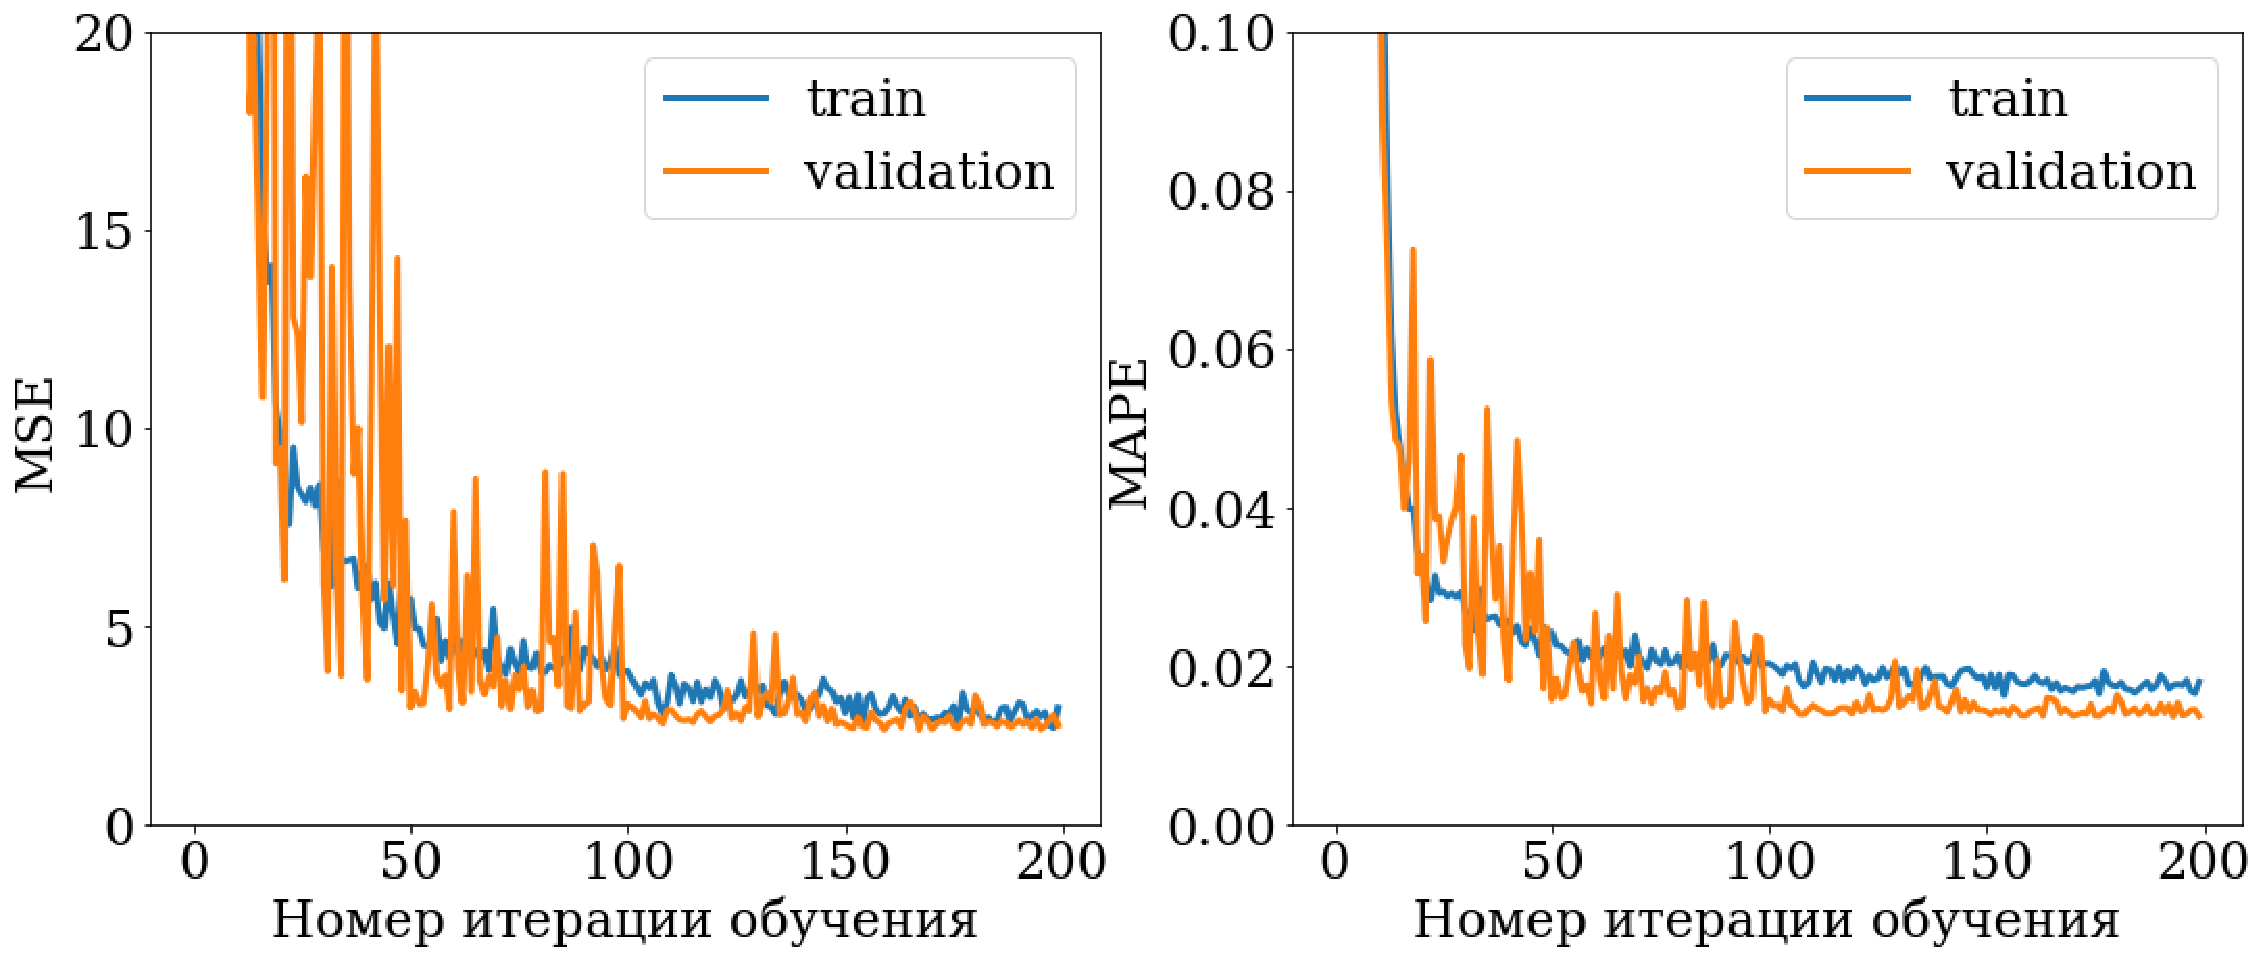
\includegraphics[scale=0.4]{img/single_experiment.pdf}
	\caption{Кривые обучения для сверточной модели.}
	\label{fig:singleexp}
\end{figure}

\subsection{Анализ ошибки}
Было проведено 50 независимых запусков эксперимента. Полученные в результате доверительные интервалы ошибки отражены на графике~\ref{fig:multerr}.
\begin{figure}[b]
	\centering
	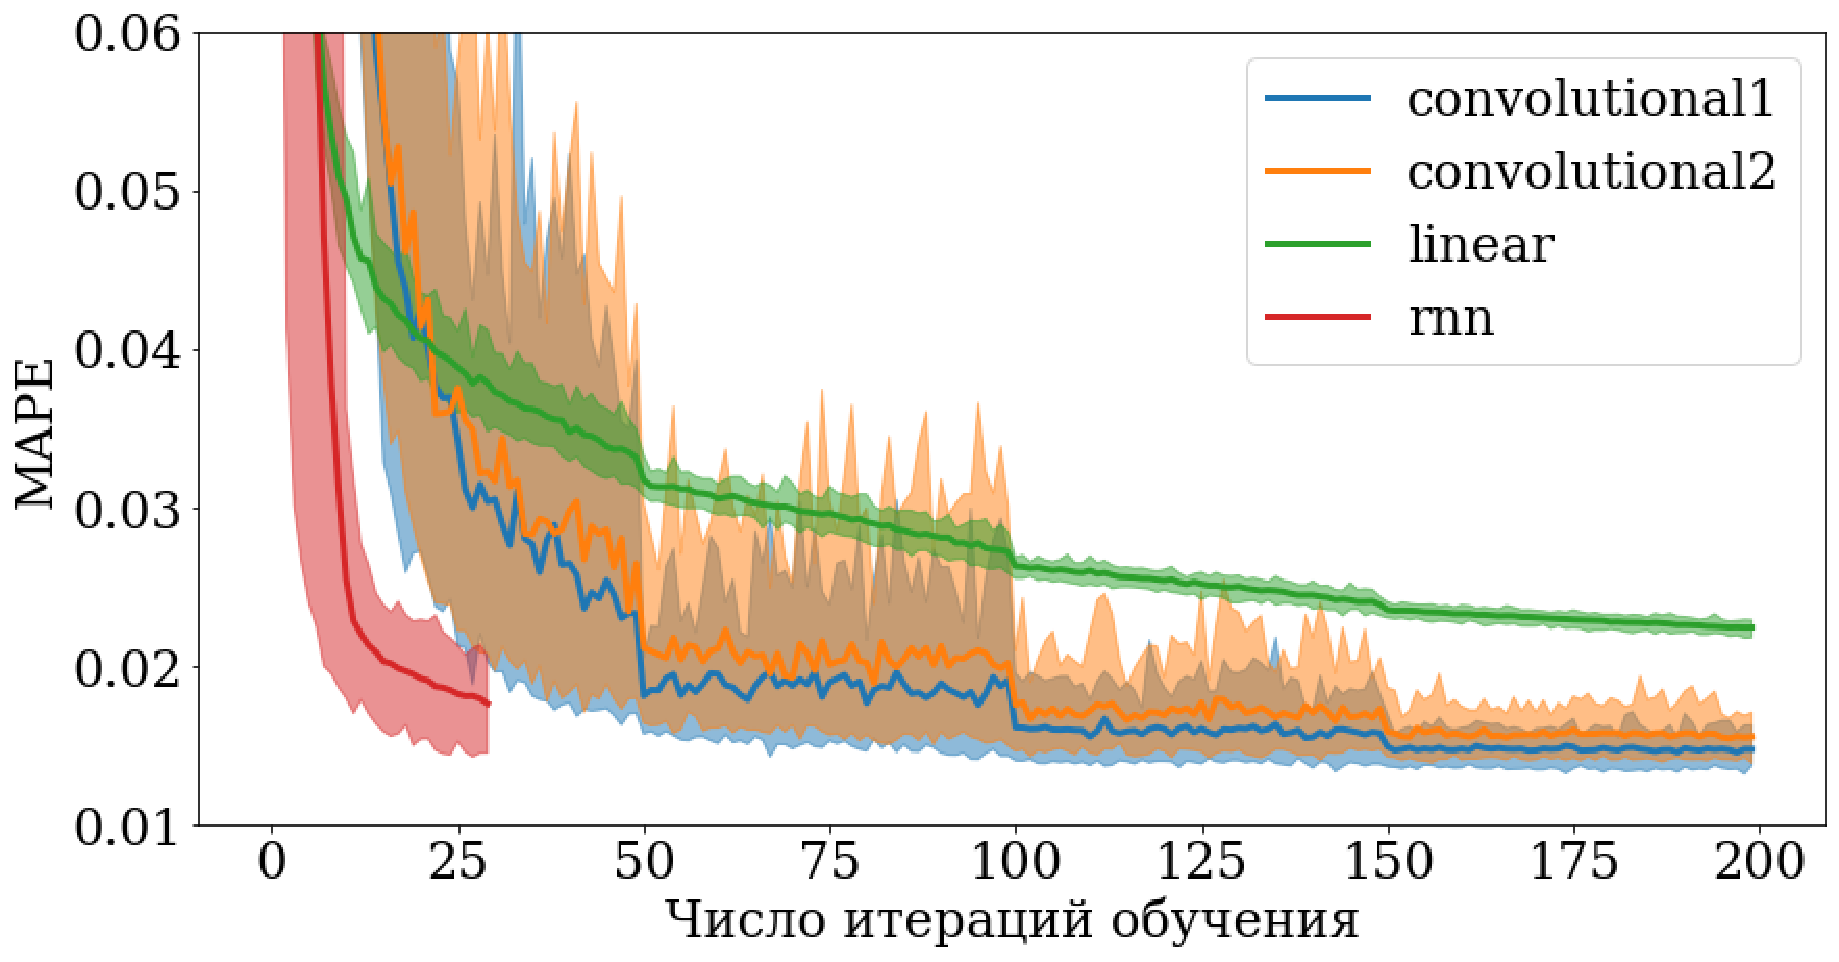
\includegraphics[scale=0.4]{img/multerror.pdf}
	\caption{Доверительный интервал ошибки на валидационной выборке.}
	\label{fig:multerr}
\end{figure}
Для каждого запуска эксперимента было посчитано итоговое качество на тестовой выборке. Результаты отображены в таблице~\ref{table:error}. По результатам эксперимента можно сказать, что реккурентная и сверточная модели хорошо справляются с обработкой круговых проекций яркости.


\begin{longtable}[]{@{}llll@{}}
\toprule
Архитектура & Число параметров & Средняя ошибка, \% & Доверительный интервал\tabularnewline
\midrule
\endhead
Полносвязная & $166402$ & $2.21$ & $2.15$-$2.24$\tabularnewline
Сверточная & $56831$\ & $1.39$ & $1.32$-$1.47$\tabularnewline
Сверточная & $17655$ & $1.48$ & $1.39$-$1.58$\tabularnewline
Реккурентная & $14962$ & $1.77$ & $1.45$-$2.05$\tabularnewline
\bottomrule
\caption{Ошибка на тестовой выборке.}
\label{table:error}
\end{longtable}

\section{Заключение}
В работе рассматривается задача поиска приблизительных границ радужки глаза. Для решения этой задачи применяется сочетание нейронной сети и метода понижения размерности~--- метода круговых проекций яркости. В результате было выявлено, что нейронные сети, созданные для обработки временных рядов, показывают точность, достаточную для первого приближения, то есть превосходящую $10\%$.

%%%% если имеется doi цитируемого источника, необходимо его указать, см. пример в \bibitem{article}
%%%% DOI публикации, зарегистрированной в системе Crossref, можно получить по адресу http://www.crossref.org/guestquery/
\begin{thebibliography}{99}


 \bibitem{article}
    \BibAuthor{A.~Nithya, C.~Lakshmi}
   Iris Recognition Techniques: A Literature Survey~//
    \BibJournal{International Journal of Applied Engineering Research}, 2015

 \bibitem{article}
    \BibAuthor{K.~Bowyer, K.~Hollingsworth, and P.~Flynn}
   Image Understanding for Iris Biometrics: A Survey~//
    \BibJournal{Computer Vision and Image Understanding}, 2008. Vol.~110. \No\,2. pp.~281--307
	
 \bibitem{article} 
    \BibAuthor{K.\,A.~Gankin, A.\,N.~Gneushev, and I.\,A.~Matveev}
   Iris image segmentation based on approximate methods
with subsequent refinements~//
    \BibJournal{Journal of Computer and Systems Sciences International}, 2014. Vol.~53. \No\,2. pp.~224--238.
	\BibDoi{10.1134/S1064230714020099}.
	
  \bibitem{article}
    \BibAuthor{I.\,A.~Matveev}
   Detection of iris in image by interrelated maxima of brightness gradient projections~//
    \BibJournal{Appl. Comput. Math.}, 2010. Vol.~9. \No\,2. pp.~252--257.
    
    \bibitem{article}
    \BibAuthor{B.~Lim, S.Zohren}
    Time-series forecasting with deep learning: a survey~//
	\BibJournal{Philosophical Transactions of the Royal Society}, A 379: 20200209.
	\BibDoi{10.1098/rsta.2020.0209}
 
 	
\end{thebibliography}

%%%% если имеется doi цитируемого источника, необходимо его указать, см. пример в \bibitem{article}
%%%% DOI публикации, зарегистрированной в системе Crossref, можно получить по адресу http://www.crossref.org/guestquery/.

\end{document}
